\subsection{ACID vs BASE}

\begin{frame}{ACID}

    Donner définition des propriétés ACID

\end{frame}

\begin{frame}{ACID vs BASE}

    \begin{figure}[htb]
        \centering
        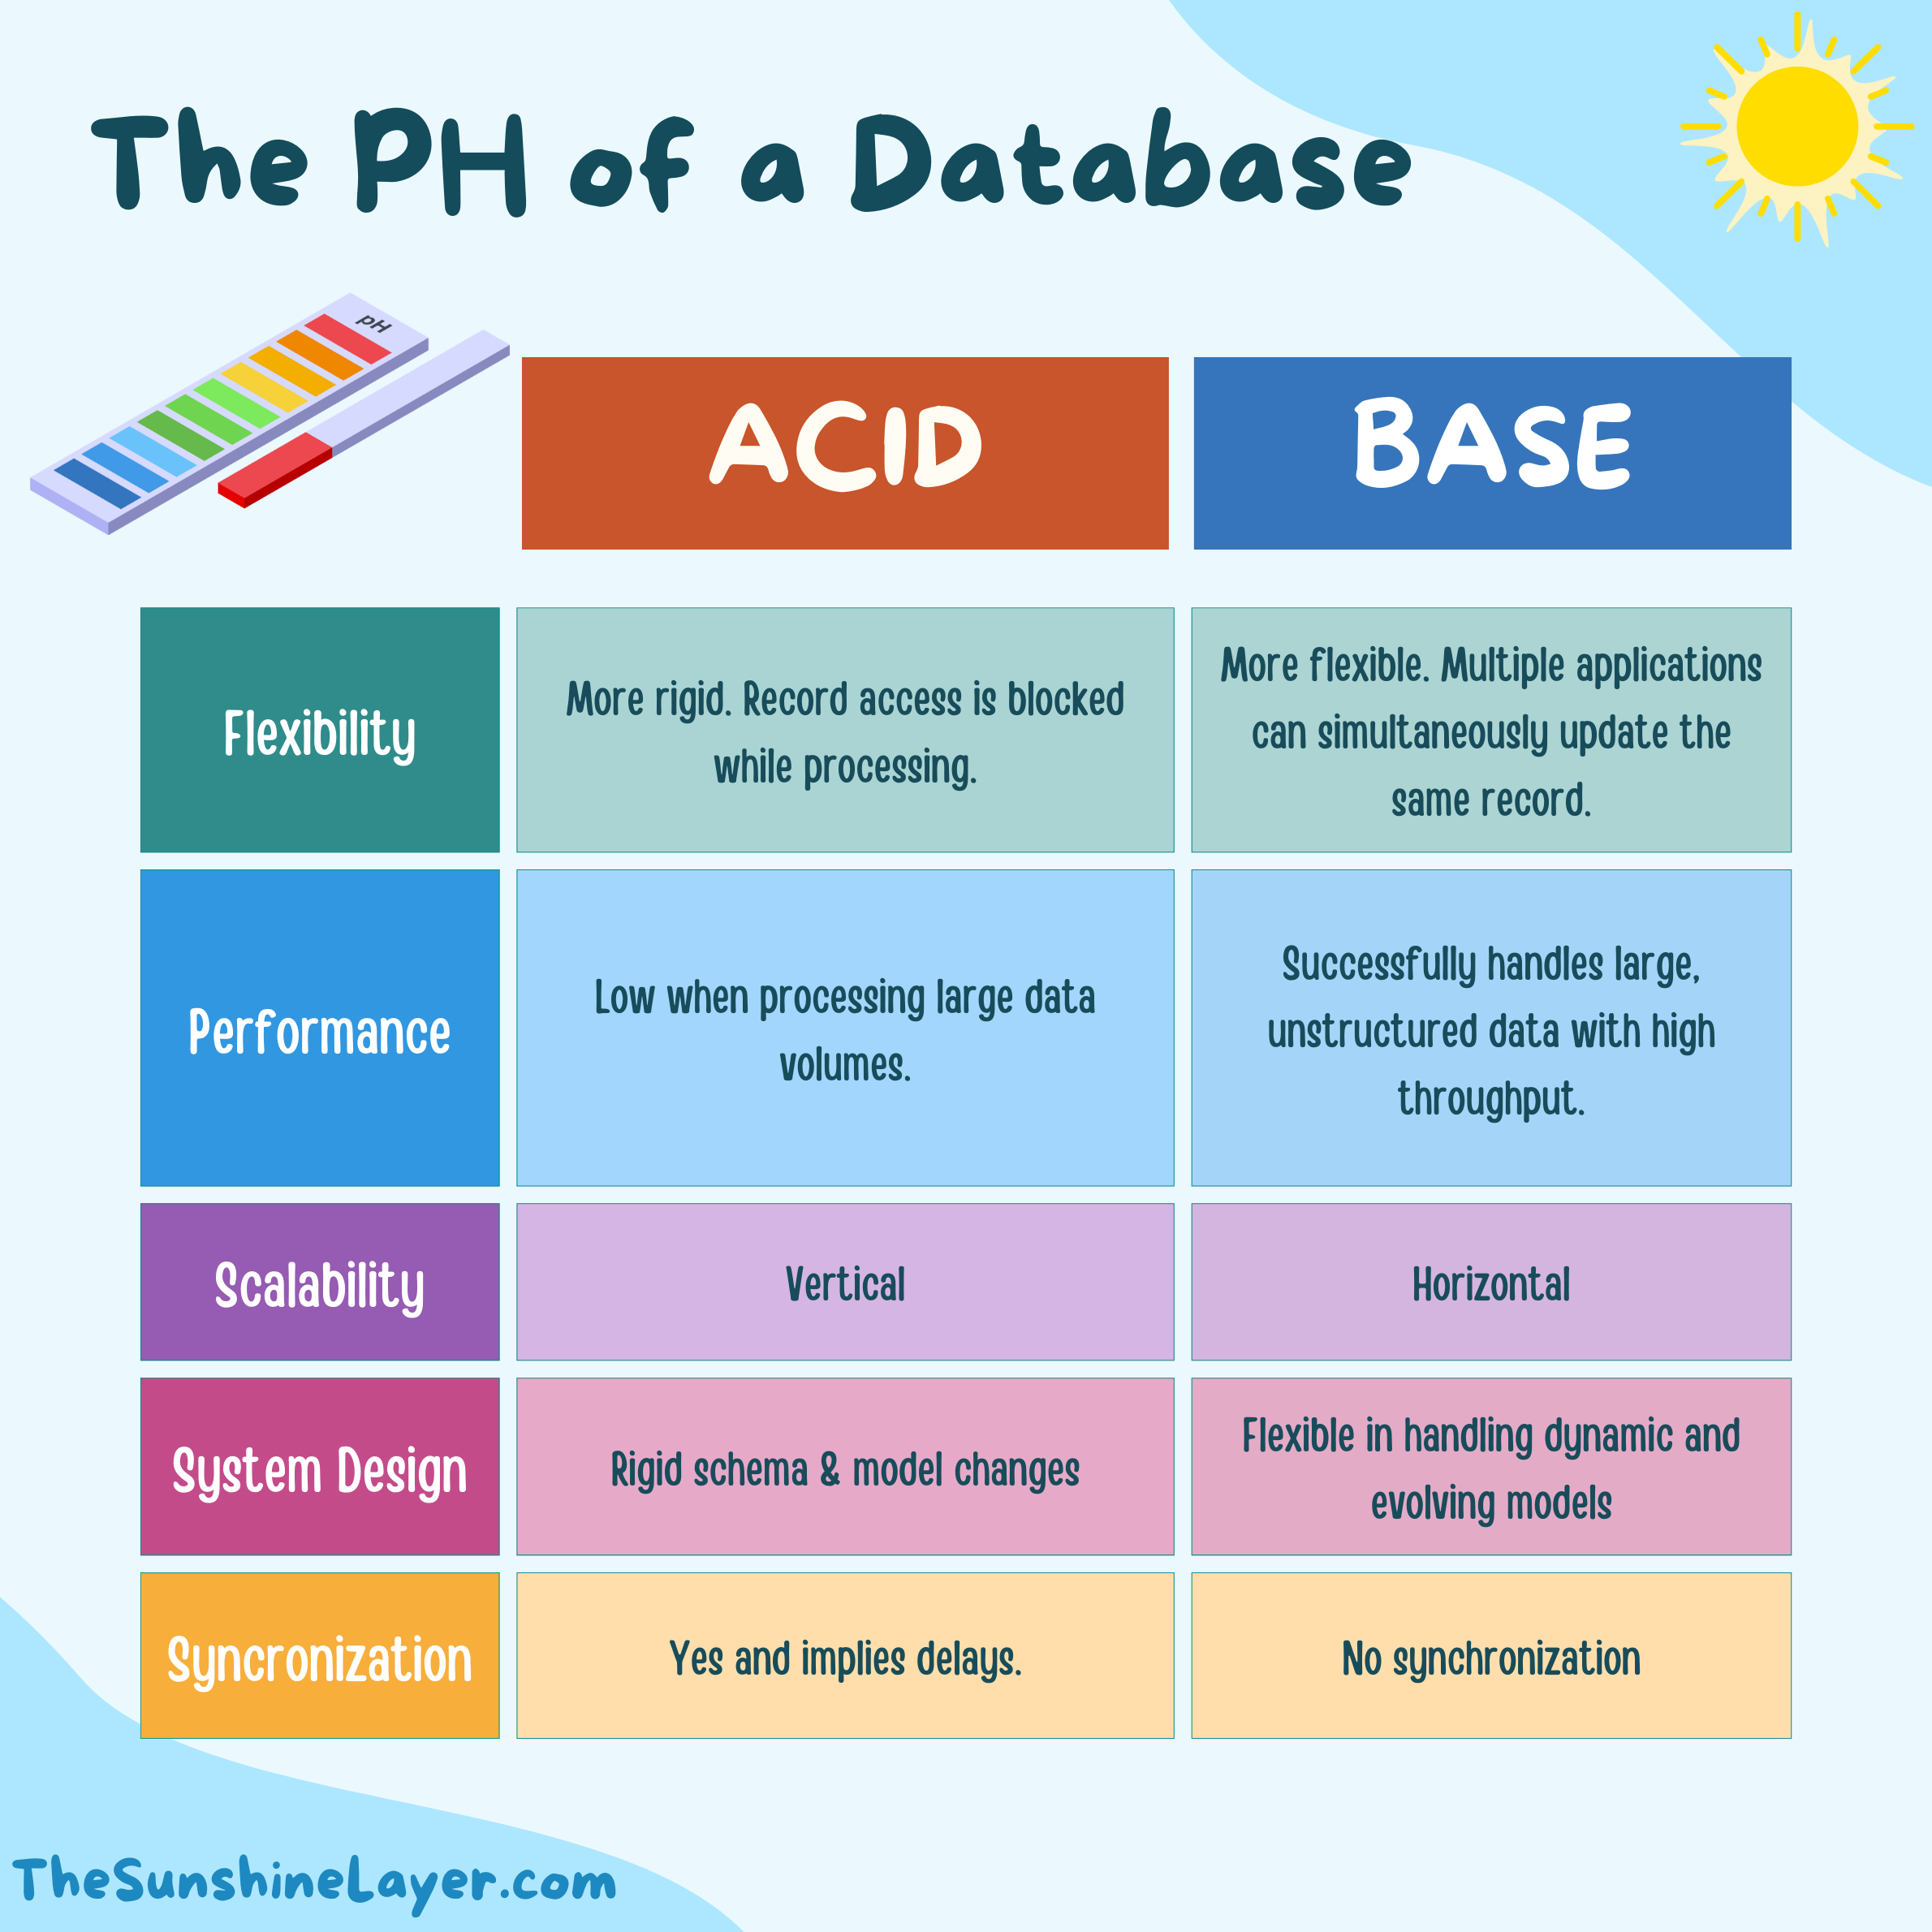
\includegraphics[height=0.9\textheight]{img/acid-vs-base.png}
    \end{figure}

\end{frame}

\begin{frame}{Transactions ACID}

    \begin{itemize}
        \item Atomicité : Toutes les opérations d'une transaction sont exécutées ou aucune
        \item Cohérence : La base de données passe d'un état valide à un autre état valide
        \item Isolation : Les transactions s'exécutent indépendamment les unes des autres
        \item Durabilité : Les modifications sont persistantes
    \end{itemize}


\end{frame}


\begin{frame}{Propriétés BASE}

    \begin{itemize}
        \item Basically Available : Le système est toujours disponible
        \item Soft state : L'état du système peut changer
        \item Eventually consistent : Le système finit par être cohérent
    \end{itemize}

\end{frame}
